\documentclass{beamer}

\usepackage[latin1]{inputenc}
\usepackage{algorithmic}
\usepackage{amsmath}
\usepackage{graphicx}
\usepackage{verbatim}

\title{Bayesian Particle Filter Tracking with CUDA}
\author{Geoffrey Ulman}
\date{May 6, 2010}
\begin{document}

%%%%%%%%%%%%%%%%%%%%%%%%%%%%%%%%%%%%%%%%%%%%%%%%%%%%

\begin{frame}
\titlepage
\end{frame}

%%%%%%%%%%%%%%%%%%%%%%%%%%%%%%%%%%%%%%%%%%%%%%%%%%%%

\begin{frame}{Motivating Example}

A submarine with a hydrophone (passive sonar) is following another
ship using the direction of the sound from the ship's engine.

\vspace{1cm}

How can the series of bearing observations from the hydrophone be
used to estimate the second ship's position and velocity?

\end{frame}

%%%%%%%%%%%%%%%%%%%%%%%%%%%%%%%%%%%%%%%%%%%%%%%%%%%%

\begin{frame}{Motivating Example}
\begin{figure}
\centering
\includegraphics[width=0.7\textwidth]{data/azimuth_only_0.png}
\end{figure}
\end{frame}

%%%%%%%%%%%%%%%%%%%%%%%%%%%%%%%%%%%%%%%%%%%%%%%%%%%%

\begin{frame}{Motivating Example}
\begin{figure}
\centering
\includegraphics[width=0.7\textwidth]{data/azimuth_only_100.png}
\end{figure}
\end{frame}

%%%%%%%%%%%%%%%%%%%%%%%%%%%%%%%%%%%%%%%%%%%%%%%%%%%%

\begin{frame}{Motivating Example}
\begin{figure}
\centering
\includegraphics[width=0.7\textwidth]{data/azimuth_only_300.png}
\end{figure}
\end{frame}

%%%%%%%%%%%%%%%%%%%%%%%%%%%%%%%%%%%%%%%%%%%%%%%%%%%%

\begin{frame}{Motivating Example}
\begin{figure}
\centering
\includegraphics[width=0.7\textwidth]{data/azimuth_only_500.png}
\end{figure}
\end{frame}

%%%%%%%%%%%%%%%%%%%%%%%%%%%%%%%%%%%%%%%%%%%%%%%%%%%%

\begin{frame}{Motivating Example}
\begin{figure}
\centering
\includegraphics[width=0.7\textwidth]{data/azimuth_only_700.png}
\end{figure}
\end{frame}

%%%%%%%%%%%%%%%%%%%%%%%%%%%%%%%%%%%%%%%%%%%%%%%%%%%%

\begin{frame}{Motivating Example}
\begin{figure}
\centering
\includegraphics[width=0.7\textwidth]{data/azimuth_only_900.png}
\end{figure}
\end{frame}

%%%%%%%%%%%%%%%%%%%%%%%%%%%%%%%%%%%%%%%%%%%%%%%%%%%%

\begin{frame}{Motivating Example}
\begin{figure}
\centering
\includegraphics[width=0.7\textwidth]{data/azimuth_only_1100.png}
\end{figure}
\end{frame}

%%%%%%%%%%%%%%%%%%%%%%%%%%%%%%%%%%%%%%%%%%%%%%%%%%%%

\begin{frame}{Motivating Example}
\begin{figure}
\centering
\includegraphics[width=0.7\textwidth]{data/azimuth_only_1300.png}
\end{figure}
\end{frame}

%%%%%%%%%%%%%%%%%%%%%%%%%%%%%%%%%%%%%%%%%%%%%%%%%%%%

\begin{frame}{Motivating Example}
\begin{figure}
\centering
\includegraphics[width=0.7\textwidth]{data/azimuth_only_1500.png}
\end{figure}
\end{frame}

%%%%%%%%%%%%%%%%%%%%%%%%%%%%%%%%%%%%%%%%%%%%%%%%%%%%

\begin{frame}{Motivating Example}
\begin{figure}
\centering
\includegraphics[width=0.7\textwidth]{data/azimuth_only_1700.png}
\end{figure}
\end{frame}

%%%%%%%%%%%%%%%%%%%%%%%%%%%%%%%%%%%%%%%%%%%%%%%%%%%%

\begin{frame}{Motivating Example}
\begin{figure}
\centering
\includegraphics[width=0.7\textwidth]{data/azimuth_only_1900.png}
\end{figure}
\end{frame}

%%%%%%%%%%%%%%%%%%%%%%%%%%%%%%%%%%%%%%%%%%%%%%%%%%%%

\begin{frame}{Motivating Example}
\begin{figure}
\centering
\includegraphics[width=0.7\textwidth]{data/azimuth_only_2100.png}
\end{figure}
\end{frame}

%%%%%%%%%%%%%%%%%%%%%%%%%%%%%%%%%%%%%%%%%%%%%%%%%%%%

\begin{frame}{Motivating Example}
\begin{figure}
\centering
\includegraphics[width=0.7\textwidth]{data/azimuth_only_2300.png}
\end{figure}
\end{frame}

%%%%%%%%%%%%%%%%%%%%%%%%%%%%%%%%%%%%%%%%%%%%%%%%%%%%

\begin{frame}{Motivating Example}
\begin{figure}
\centering
\includegraphics[width=0.7\textwidth]{data/azimuth_only_2500.png}
\end{figure}
\end{frame}

%%%%%%%%%%%%%%%%%%%%%%%%%%%%%%%%%%%%%%%%%%%%%%%%%%%%

\begin{frame}{Motivating Example}
\begin{figure}
\centering
\includegraphics[width=0.7\textwidth]{data/azimuth_only_2700.png}
\end{figure}
\end{frame}

%%%%%%%%%%%%%%%%%%%%%%%%%%%%%%%%%%%%%%%%%%%%%%%%%%%%

\begin{frame}{Motivating Example}
\begin{figure}
\centering
\includegraphics[width=0.7\textwidth]{data/azimuth_only_2900.png}
\end{figure}
\end{frame}

%%%%%%%%%%%%%%%%%%%%%%%%%%%%%%%%%%%%%%%%%%%%%%%%%%%%

\begin{frame}{Motivating Example}
\begin{figure}
\centering
\includegraphics[width=0.7\textwidth]{data/azimuth_only_3100.png}
\end{figure}
\end{frame}

%%%%%%%%%%%%%%%%%%%%%%%%%%%%%%%%%%%%%%%%%%%%%%%%%%%%

\begin{frame}{Motivating Example}
\begin{figure}
\centering
\includegraphics[width=0.7\textwidth]{data/azimuth_only_3300.png}
\end{figure}
\end{frame}

%%%%%%%%%%%%%%%%%%%%%%%%%%%%%%%%%%%%%%%%%%%%%%%%%%%%

\begin{frame}{Motivating Example}
\begin{figure}
\centering
\includegraphics[width=0.7\textwidth]{data/azimuth_only_3500.png}
\end{figure}
\end{frame}

%%%%%%%%%%%%%%%%%%%%%%%%%%%%%%%%%%%%%%%%%%%%%%%%%%%%

\begin{frame}{Motivating Example}
\begin{figure}
\centering
\includegraphics[width=0.7\textwidth]{data/azimuth_only_3700.png}
\end{figure}
\end{frame}

%%%%%%%%%%%%%%%%%%%%%%%%%%%%%%%%%%%%%%%%%%%%%%%%%%%%

\begin{frame}{Motivating Example}
\begin{figure}
\centering
\includegraphics[width=0.7\textwidth]{data/azimuth_only_4000.png}
\end{figure}
\end{frame}

%%%%%%%%%%%%%%%%%%%%%%%%%%%%%%%%%%%%%%%%%%%%%%%%%%%%

\begin{frame}{Likelihood Function}
\begin{equation}
L(y|x) = P( Y=y | X=x ) \hspace{0.5cm} \mbox{for} \hspace{0.5cm} x \in S
\end{equation}

\vspace{1cm}

\begin{itemize}
\item \(X\) Random variable on \(S\)
\item \(Y\) Random variable on measurement space \(H\)
\item \(P(\cdot|x)\) Probability density function on \(H\)
\item \(P(y|\cdot)\) Likelihood function relating \(X\) and \(Y\)
\end{itemize}

\end{frame}


%%%%%%%%%%%%%%%%%%%%%%%%%%%%%%%%%%%%%%%%%%%%%%%%%%%%

\begin{frame}{Likelihood Function}

Why is \(P(y|\cdot)\) called a "Likelihood Function"?

\vspace{1cm}

For \hspace{0.25cm} \(x_{1}, x_{2} \in S \) \hspace{0.25cm} if \hspace{0.25cm} \(L(y|x_{1})>L(y|x_{2})\) \hspace{0.25cm} then:

\vspace{1cm}

The observation \(y\) is more likely to have come from a target with state \(x_{1}\) than a target with state \(x_{2}\)

\end{frame}

%%%%%%%%%%%%%%%%%%%%%%%%%%%%%%%%%%%%%%%%%%%%%%%%%%%%

\begin{frame}{Likelihood Function}

\[
L(y|x_{1})>L(y|x_{2})
\]

\begin{figure}
\centering
\includegraphics[width=0.6\textwidth]{data/likelihood_function_diagram.png}
\end{figure}

\end{frame}

%%%%%%%%%%%%%%%%%%%%%%%%%%%%%%%%%%%%%%%%%%%%%%%%%%%%

\begin{frame}{Bayes' Rule}

Reverand Thomas Bayes (1702-1761):

\vspace{1cm}

\begin{equation}
P(A|B)=\frac{P(B|A)P(A)}{P(B)}
\end{equation}

\end{frame}

%%%%%%%%%%%%%%%%%%%%%%%%%%%%%%%%%%%%%%%%%%%%%%%%%%%%

\begin{frame}{Bayesian Inference}

\begin{equation}
P(x|y) = \frac{L(y|x)P(x)}{P(y)} = \frac{L(y|x)P(x)}{\int \! L(y|x)P(x) \, dx}
\end{equation}

\vspace{1cm}

\begin{itemize}
\item Observation \(y\) is fixed, \(x\) represents possible target states
\item \(P(x)\) Prior probability density function on true target state
\item \(P(x|y)\) Posterior distribution given observation \(y\)
\end{itemize}

\vspace{1cm}

\emph{"Multiply each particle's weight by the likelihood function evaluated at the particle then normalize by the sum over all particle weights."}

\end{frame}

%%%%%%%%%%%%%%%%%%%%%%%%%%%%%%%%%%%%%%%%%%%%%%%%%%%%


\begin{frame}{Prior Distribution}

\begin{figure}
\centering
\includegraphics[width=0.7\textwidth]{data/particles_prior.png}
\caption{Prior Particle Position Distribution}
\end{figure}

\end{frame}


%%%%%%%%%%%%%%%%%%%%%%%%%%%%%%%%%%%%%%%%%%%%%%%%%%%%


\begin{frame}{Information Update}

\begin{figure}
\centering
\includegraphics[width=0.7\textwidth]{data/particles_azimuth_obs.png}
\caption{Posterior Particle Position Distribution after Azimuth Observation}
\end{figure}

\end{frame}


%%%%%%%%%%%%%%%%%%%%%%%%%%%%%%%%%%%%%%%%%%%%%%%%%%%%


\begin{frame}{Resampling}

\begin{equation}\label{resample1}
C = \frac{n}{\sum_{i=0}^{n} w_{i}}
\end{equation}

\vspace{0.5cm}

\begin{itemize}
\item \(C\) Normalizing constant
\item \(w_{i}\) Particle weights
\item \(n\) Number of particles
\end{itemize}

\vspace{0.5cm}

\begin{center}
Example \(w_{i}\) Array:
\end{center}

\renewcommand{\tabcolsep}{0.5cm}
\begin{center}
\begin{tabular}{ | c | c | c | c | c | }
  \hline
   0.8 & 0.4 & 6.6 & 0.6 & 1.6 \\
  \hline
\end{tabular}
\end{center}

\begin{center}
\(C = \frac{5}{10} = 0.5 \)
\end{center}

\end{frame}


%%%%%%%%%%%%%%%%%%%%%%%%%%%%%%%%%%%%%%%%%%%%%%%%%%%%

\begin{frame}{Resampling}

\begin{equation}\label{resample2}
\overline{w}_{i}=C w_{i}
\end{equation}

\vspace{0.5cm}

\begin{center}
Example \(\overline{w}_{i}\) Array:
\end{center}

\renewcommand{\tabcolsep}{0.5cm}
\begin{center}
\begin{tabular}{ | c | c | c | c | c | c | }
  \hline
   0.4 & 0.2 & 3.3 & 0.3 & 0.8 \\
  \hline
\end{tabular}
\end{center}

\end{frame}


%%%%%%%%%%%%%%%%%%%%%%%%%%%%%%%%%%%%%%%%%%%%%%%%%%%%

\begin{frame}{Resampling}

\begin{equation}\label{resample3}
\hat{w}_{i}=\operatorname{floor}(\sum_{j=0}^{i} \overline{w}_{j})
\end{equation}

\vspace{0.5cm}

\begin{center}
Example \(\hat{w}_{i}\) Array:
\end{center}

\renewcommand{\tabcolsep}{0.5cm}

\begin{center}
Cumulative Sums:
\end{center}
\begin{center}
\begin{tabular}{ | c | c | c | c | c | c | }
  \hline
   0.4 & 0.6 & 3.9 & 4.2 & 5.0 \\
  \hline
\end{tabular}
\end{center}

\renewcommand{\tabcolsep}{0.65cm}

\begin{center}
Floor:
\end{center}
\begin{center}
\begin{tabular}{ | c | c | c | c | c | c | }
  \hline
   0 & 0 & 3 & 4 & 5 \\
  \hline
\end{tabular}
\end{center}

\end{frame}

%%%%%%%%%%%%%%%%%%%%%%%%%%%%%%%%%%%%%%%%%%%%%%%%%%%%

\begin{frame}[containsverbatim]{Parallel Summation}

\begin{figure}
\centering
\includegraphics[width=0.7\textwidth]{data/summation.png}
\caption{Prior Particle Position Distribution}
\end{figure}

\end{frame}

%%%%%%%%%%%%%%%%%%%%%%%%%%%%%%%%%%%%%%%%%%%%%%%%%%%%

\begin{frame}[containsverbatim]{Parallel Summation}


 \begin{verbatim}
  __shared__ float s_shared[ blockDim.x ];
  int tid = threadIdx.x;
  unsigned int offset = blockDim.x / 2;

  while ( offset > 0 )
  {
    if ( tid < offset )
    {
      s_shared[ tid ] += s_shared[ tid + offset ];
    }

    offset = offset >> 1; // divide offset by 2

    __syncthreads();
  }
 \end{verbatim}

\end{frame}

%%%%%%%%%%%%%%%%%%%%%%%%%%%%%%%%%%%%%%%%%%%%%%%%%%%%

\begin{frame}[containsverbatim]{Parallel Summation Improved}

 \begin{verbatim}
  ...

  while ( offset > 32 )
  {
    ...
  }

  if ( tid < 32 )
  {
    s_shared[ tid ] += s_shared[ tid + 32 ];
    s_shared[ tid ] += s_shared[ tid + 16 ];
    s_shared[ tid ] += s_shared[ tid + 8 ];
    s_shared[ tid ] += s_shared[ tid + 4 ];
    s_shared[ tid ] += s_shared[ tid + 2 ];
    s_shared[ tid ] += s_shared[ tid + 1 ];
  }

 \end{verbatim}

\end{frame}

%%%%%%%%%%%%%%%%%%%%%%%%%%%%%%%%%%%%%%%%%%%%%%%%%%%%

\begin{frame}{Resampling Results}

\begin{figure}
\centering
\includegraphics[width=1.0\textwidth]{data/profile_cuda_version1_pic1.png}
\caption{CUDA Visual Profiler Version 1 Results}
\end{figure}

\end{frame}

%%%%%%%%%%%%%%%%%%%%%%%%%%%%%%%%%%%%%%%%%%%%%%%%%%%%

\begin{frame}{Improved Resampling Results}

\begin{figure}
\centering
\includegraphics[width=1.0\textwidth]{data/profile_cuda_version2_pic1.png}
\caption{CUDA Visual Profiler Version 2 Results}
\end{figure}

\end{frame}

%%%%%%%%%%%%%%%%%%%%%%%%%%%%%%%%%%%%%%%%%%%%%%%%%%%%

\begin{frame}{Performance}

\begin{figure}
\centering
\includegraphics[width=0.85\textwidth]{data/timing_results.png}
\label{final_timing1}
\end{figure}

\end{frame}

%%%%%%%%%%%%%%%%%%%%%%%%%%%%%%%%%%%%%%%%%%%%%%%%%%%%

\begin{frame}{Performance}

\begin{figure}
\centering
\includegraphics[width=0.85\textwidth]{data/timing_results_speedup.png}
\label{final_timing2}
\end{figure}

\end{frame}

%%%%%%%%%%%%%%%%%%%%%%%%%%%%%%%%%%%%%%%%%%%%%%%%%%%%

\begin{frame}{Lessons Learned}

\begin{itemize}
\item CUDA optimization is \emph{hard}
\begin{itemize}
\item Uncoalesced memory access
\item Shared memory bank conflicts
\item Slow operators (like modulus)
\end{itemize}
\item However, even codes with the above problems can achieve significant speedup
\item CUDA Visual Profiler
\begin{itemize}
\item useful and user friendly
\end{itemize}
\item thrust
\begin{itemize}
\item fast and well documented
\end{itemize}
\end{itemize}


\end{frame}

%%%%%%%%%%%%%%%%%%%%%%%%%%%%%%%%%%%%%%%%%%%%%%%%%%%%

\begin{frame}{Backup Slides}

Backup Slides

\end{frame}

%%%%%%%%%%%%%%%%%%%%%%%%%%%%%%%%%%%%%%%%%%%%%%%%%%%%

\begin{frame}{Effective Particle Count}

\begin{equation}
\overline{w}_{i} = \frac{w_{i}}{\sum_{i=1}^{n} w_{i}}
\end{equation}

\vspace{0.2cm}

\begin{equation}
N_{eff} = \frac{1}{\sum_{i=1}^{n} \overline{w}_{i}^2}
\end{equation}

\vspace{1cm}

\begin{center}

For \hspace{0.3cm} \(\overline{w}_{i}=\frac{1}{n}\) \hspace{2.4cm} \(N_{eff} = \frac{1}{n\frac{1}{n^2}} = n \)

\vspace{1cm}

For \hspace{0.3cm} \(
\overline{w}_{i} = \begin{cases}

  1 & \text{for $i=0$} \\

  0 & \text{otherwise}

\end{cases}
\)\hspace{0.4cm} \(N_{eff} = \frac{1}{1} = 1 \)

\end{center}

\end{frame}

%%%%%%%%%%%%%%%%%%%%%%%%%%%%%%%%%%%%%%%%%%%%%%%%%%%%

\end{document}
